%travail_decorator
\subsection{Décorateur}
\begin{figure}[h]
\begin{center}
    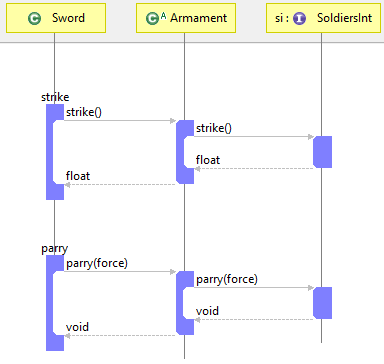
\includegraphics[width=11cm]{diagSeqDecorator}
\end{center}
    \caption{Diagramme de séquence du pattern décorateur}
    \label{sequence-decorateur}
\end{figure}

La première étape de conception du projet consistait en l'implémentation de soldats disposant d'armements (un bouclier et une épée par exemple). Nous disposions de deux catégories de soldats : les fantassins et les cavaliers. Les soldats possédaient un certain nombre de points de vie.

Pour réaliser cette première étape, nous avons commencé par créer les deux classes de soldats ainsi que deux classes d'armes. Afin d'anticiper le fait de pouvoir rajouter plus de catégories de soldat et plus d'armes, nous avons créé deux classes abstraites : \emph{Armament} et \emph{SoldierAbstract}.  

L'objectif était alors de pouvoir rajouter une ou plusieurs armes sur un soldat de façon dynamique, c'est-à-dire sans avoir à recréer le soldat. 

Pour répondre à cette problématique, nous avons utilisé le pattern \emph{Décorateur}. 
Nous avons donc créé une interface \emph{SoldierInt} associée aux soldats. Nous avons ensuite fait implémenter notre interface \emph{SoldierInt} par nos classes \emph{SoldierAbstract} et \emph{Armament}. \emph{Armament} devenant notre décorateur puisque nous avons rajouté dans cette classe une délégation sur un \emph{SoldierInt}, ce qui permet de décorer notre soldat, voir la figure \vref{sequence-decorateur}.

Ainsi donc, nous pouvons maintenant décorer un soldat avec des armes.

Une autre architecture possible aurait été de séparer les armes des soldats, ceci en créant un décorateur \emph{SoldierArmed} avec comme sous-classe \emph{SoldierWithShield} et \emph{SoldierWithSword}. Ceci permettrait de séparer le comportement des armes du comportement des soldats, pour ainsi définir des méthodes spécifiques aux armes sans affecter les soldats, et inversement. Cette solution a pour inconvénient de nécessiter l'ajout d'un nombre de classes croissant avec le nombre d'armements implémentés.

Une fois notre première architecture créée, nous avons rajouté la possibilité pour un soldat de porter des coups à ses adversaires (et à contrario de les parer) avec une vivacité dépendant de l'armement et de la catégorie du soldat.